%%%%%%%%%%%%%%%%%%%%%%%%%%%%%%%%%%%%%%%%%
% Journal Article
% LaTeX Template
% Version 1.4 (15/5/16)
%
% This template has been downloaded from:
% http://www.LaTeXTemplates.com
%
% Original author:
% Frits Wenneker (http://www.howtotex.com) with extensive modifications by
% Vel (vel@LaTeXTemplates.com)
%
% License:
% CC BY-NC-SA 3.0 (http://creativecommons.org/licenses/by-nc-sa/3.0/)
%
%%%%%%%%%%%%%%%%%%%%%%%%%%%%%%%%%%%%%%%%%

%----------------------------------------------------------------------------------------
%	PACKAGES AND OTHER DOCUMENT CONFIGURATIONS
%----------------------------------------------------------------------------------------

\documentclass[twoside,twocolumn]{article}

\usepackage[sc]{mathpazo} % Use the Palatino font
\usepackage[T1]{fontenc} % Use 8-bit encoding that has 256 glyphs
\linespread{1.05} % Line spacing - Palatino needs more space between lines
\usepackage{microtype} % Slightly tweak font spacing for aesthetics

\usepackage[english]{babel} % Language hyphenation and typographical rules

\usepackage[hmarginratio=1:1,top=32mm,columnsep=20pt]{geometry} % Document margins
\usepackage[hang, small,labelfont=bf,up,textfont=it,up]{caption} % Custom captions under/above floats in tables or figures
\usepackage{booktabs} % Horizontal rules in tables

\usepackage{lettrine} % The lettrine is the first enlarged letter at the beginning of the text

\usepackage{enumitem} % Customized lists

\usepackage{abstract} % Allows abstract customization
\renewcommand{\abstractnamefont}{\normalfont\bfseries} % Set the "Abstract" text to bold
\renewcommand{\abstracttextfont}{\normalfont\small\itshape} % Set the abstract itself to small italic text

\usepackage{titlesec} % Allows customization of titles
\renewcommand\thesection{\Roman{section}} % Roman numerals for the sections
\renewcommand\thesubsection{\roman{subsection}} % roman numerals for subsections


\usepackage{fancyhdr} % Headers and footers
\pagestyle{fancy} % All pages have headers and footers
\fancyhead{} % Blank out the default header
\fancyfoot{} % Blank out the default footer
\fancyhead[C]{Analysis of Gravitation $\bullet$ May 2017} % Custom header text
\fancyfoot[RO,LE]{\thepage} % Custom footer text

\usepackage{titling} % Customizing the title section

\usepackage{hyperref} % For hyperlinks in the PDF

\usepackage{graphicx}
\usepackage{float}
\usepackage{amsmath}
\usepackage{empheq}

\graphicspath{ {graphics/} }

%----------------------------------------------------------------------------------------
%	TITLE SECTION
%----------------------------------------------------------------------------------------

\title{Analysis of Gravitation: Measuring the Gravitational Constant G} % Article title
\author{
\textsc{Gabriel Smadi} \\ % Your name
\normalsize{Syracuse University} \\ % Your institution
\normalsize \href{mailto:gsmadi@syr.edu}{gsmadi@syr.edu} % Your email address
}

\date{\today} % Leave empty to omit a date

%----------------------------------------------------------------------------------------

\begin{document}

% Print the title
\maketitle

\begin{abstract}
  A modern version of Henry Cavendish's experiment is carried out in order to measure the universal
  constant of gravitation G. Using a torsion balance and some creative configurations the necessary
  values to compute G are measured and an estimate is obtained. The value of G is measured with 15$\%$ error.
\end{abstract}

%----------------------------------------------------------------------------------------
%	ARTICLE CONTENTS
%----------------------------------------------------------------------------------------

\section{Introduction}

When Isaac Newton derived the Law of universal gravitation, the constant Ghad still never been
measured. After Newton came Henry Cavendish with an ingenius procedure to measure the elusive constant
at the time. Cavendish performed his experiment with a torsion balance and some mirrors. After succesfully
measuring the constant G, Cavendish wittingly suggested he had measured the "weight of the earth". We shall
perform Cavendish's famous experiment in a more modern setting.

%------------------------------------------------

\section{Methods}

The main component in the experiment is the torsion balance apparatus as seen in Figure 1. Inside the
apparatus, there is a rod with two small lead balls of mass $m_{1}$ at each end. Outside the apparatus there is
a pivoting support with two larger lead balls of mass $m_{2} = 1.5$ kg.

\begin{figure}[H]
\centering
  \begin{center}
    \scalebox{.3}{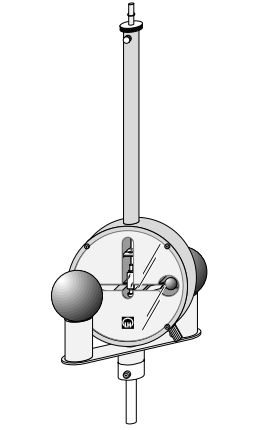
\includegraphics{apparatus}}
  \end{center}
  \caption{Main apparatus of the experiment}
\end{figure}
\label{fig:apparatus}

Two of the masses will have a small interacting force given by,

\begin{equation}
\label{eq:attraction}
F = G \mult \frac{m_{1}m_{2}}{b^2}
\end{equation}

where $b = 47$ mm is the distance from $m_{1}$ to $m_{2}$.

Since the torsion balance is free to rotate, it shall experience a torque as,

\begin{equation}
\label{eq:torque}
\tau_{I} = F_{net} \times r = (2F) \mult d = 2G \mult \frac{m_{1}m_{2}d}{b^2}
\end{equation}

where $d = 50$ mm is the radius of the torsion balance.

As the pivoting support is rotated between Position I and Position II, the torsion balance will experience
a torque in each position. Thus, both torques can be related as,

\begin{equation}
\label{eq:pos_torque}
\tau_{I} = -\tau_{II} = \kappa \theta
\end{equation}

The motion of the torsion balance is given by the following differential equation,

\begin{equation}
\label{eq:diff_eq}
  I\frac{d^2\theta}{dt^2} + D\frac{d\theta}{dt} + \kappa \theta = 0
\end{equation}

where $\kappa$ is the torsion constant and D the damping factor. A solution to the differential
equation,

\begin{equation}
\label{eq:diff_sol}
\theta(t) = \theta_{0}cos(\omega t + \phi)e^{-\frac{t}{\tau}} + C
\end{equation}

where $\tau = 1 / \kappa $. The period of rotation for the rigid rod is,

\begin{equation}
\label{eq:period}
T = 2\pi \mult \sqrt{\frac{I}{\kappa}}
\end{equation}

where for a rigid rod the moment of inertia is given by,

\begin{equation}
\label{eq:inertia}
I = m_{2}(\frac{d}{2})^2 + m_{2}(\frac{d}{2})^2 = \frac{m_{2}d^2}{2}
\end{equation}

Thus, from Equation \ref{eq:period} we solve for the torsion constant such that,

\begin{equation}
\label{eq:kappa}
\kappa = \frac{2m_{2}d^2\pi^2}{T^2}
\end{equation}

After sometime the torsion balance rotations will die out and settle into an equilibrium state illustrated in
Figure 2.

\begin{figure}[H]
\centering
  \begin{center}
    \scalebox{.5}{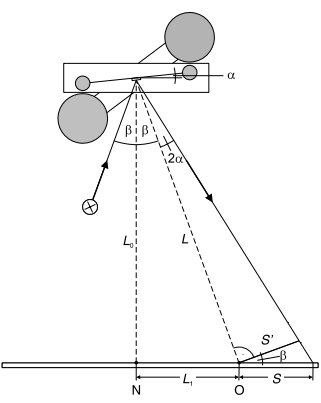
\includegraphics{geometry}}
  \end{center}
  \caption{Geometric configuration of the experiment}
\end{figure}
\label{fig:geometry}

Using a laser pointer and a mirror mounted on the torsion balance we may extract the oscillatory
$\theta(t)$ from Equation \ref{eq:diff_sol}. The glass ruler to obtain the reflected point from the laser
pointer is at a distance $L_{0}$. The distance from the N position on the ruler to the equilibrium position
of the laser pointer without both $m_{1}$ masses is given by $L_{1}$.

Let $\theta = (\alpha_{I} - \alpha_{II})$, which is the difference between the equilibrium angles
of the torsion balance. The net torque exerted on the torsion balance by both torques is equal to,

\begin{equation}
\label{eq:net_roque}
\tau_{net} = Fd = \kappa\theta
\end{equation}

$\Rightarrow$
$$
  (\frac{Gm_{1}m_{2}}{b^2}) \mult d = \kappa (\alpha_{I} - \alpha_{II})
$$

$\Rightarrow$
$$
  (\frac{Gm_{1}m_{2}}{b^2}) \mult d = (\frac{2m_{2}d^2\pi^2}{T^2}) \mult (\alpha_{I} - \alpha_{II})
$$

$\Rightarrow$

\begin{equation}
\label{eq:almost_g}
G = \frac{2\pi^{2}db^2}{m_{1}T^2} \mult (\alpha_{I} - \alpha_{II})
\end{equation}

By inspecting the geometry of the configuration in Figure 2, we find that,

$$
  \alpha_{I} = \frac{S_{I}}{2} \mult \frac{L_{0}}{L_{0}^2 + L_{1}^2}, \quad
  \alpha_{II} = \frac{S_{II}}{2} \mult \frac{L_{0}}{L_{0}^2 + L_{1}^2}
$$

where $S_{I}$ and $S_{II}$ are the equilibrium distances of the laser pointer on the ruler for both
Position I and Position II configurations, respectively.

$\Rightarrow$

\begin{equation}
\label{eq:delta_alpha}
  (\alpha_{I} - \alpha_{II}) = \frac{(S_{I} - S_{II})}{2} \mult \frac{L_{0}}{L_{0}^2 + L_{1}^2}}
\end{equation}

Therefore, by Eq. \ref{eq:almost_g} and Eq. \ref{eq:delta_alpha} our final equations for G is,

\begin{equation}
\label{eq:final_g}
  \boxed{G = \frac{\pi^{2}b^2d}{m_{1}} \mult \frac{(S_{I} - S_{II})}{T^2} \mult \frac{L_{0}}{L_{0}^2 + L_{1}^2}}
\end{equation}

All values in the above equation are either given or measurable, hence G can be computed.

%------------------------------------------------

\section{Results}

Measuring the distance from the torsion balance to the glass ruler,

\begin{equation}
\label{eq:l_0}
L_{0} = 2.13 \pm 0.012 \quad m
\end{equation}

Similarly measuring the equilibrium position $L_{1}$,

\begin{equation}
\label{eq:l_1}
L_{1} = 5.2 \pm 0.1 \quad cm
\end{equation}

By obtaining the amplitudes of the torsion balance as a function of time we may find
the period and equilibriums. To fit the aquired data the following fit function was used
in similar form to Equation \ref{eq:diff_sol},

\begin{equation}
\label{eq:diff_sol}
\y_{fit}(t) = Acos(\frac{2\pi}{T} t + \phi)e^{-\frac{t}{\tau}} + C
\end{equation}

We note from the fit function that are equilibrium positions $S_{I}$ and $S_{II}$ are given by
the offset C in the fit function.

\begin{figure}[H]
\centering
  \begin{center}
    \scalebox{.5}{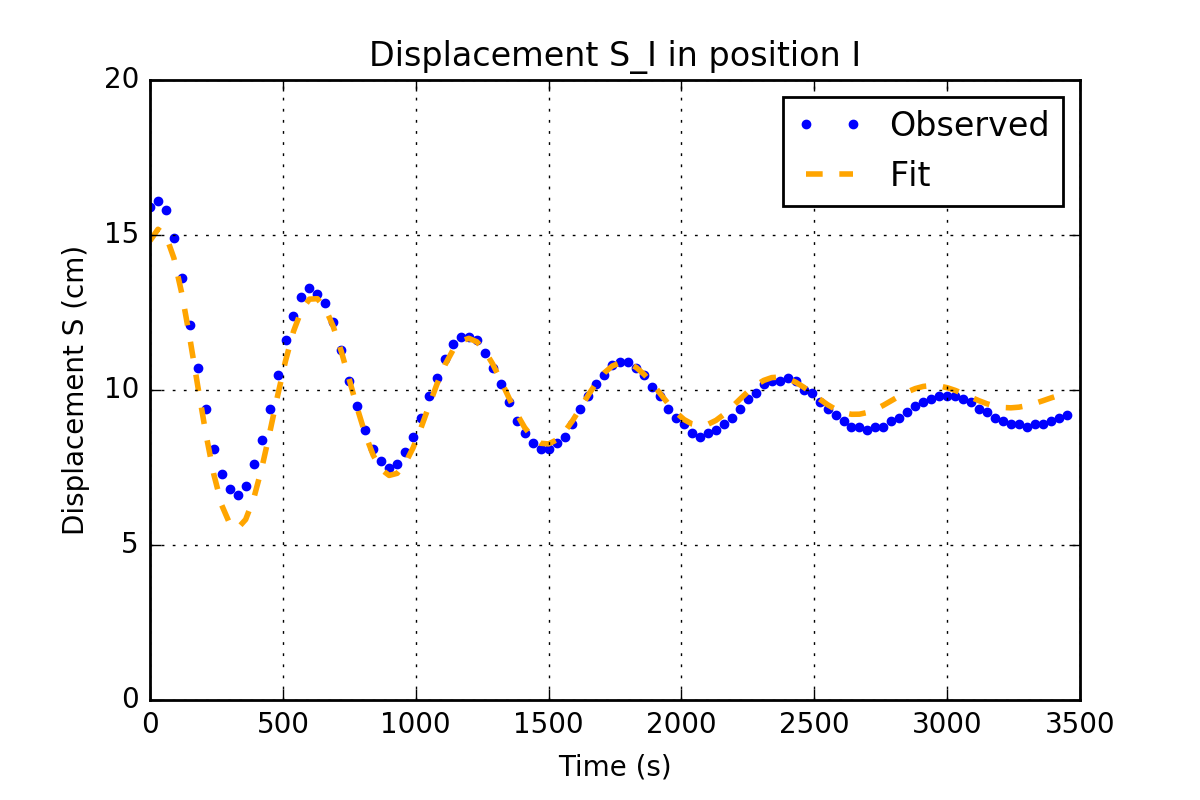
\includegraphics{pos1_datafit}}
  \end{center}
  \caption{Data points and fit function for Position I data}
\end{figure}
\label{fig:pos1_plot}

Fitting the data using least squares fitting routine we obtain the optimized
parameters as seen in Table 1.

\begin{table}[H]
\centering
\begin{tabular}{llr}
\toprule
\cmidrule(r){1-2}
Parameter & Value \\
\midrule
$ A$ & $ 5.6 \pm 0.2 $ \\
$ \tau$ & $ 1120 \pm 61 $ \\
$ T$ & $ 582 \pm 3 $ \\
$ \phi$ & $ -0.45 \pm 0.04 $ \\
$ C$ & $ 9.74 \pm 0.04 $ \\
\bottomrule
\end{tabular}
\caption{Optimized fit function parameters for Position I}
\end{table}

\begin{figure}[H]
\centering
  \begin{center}
    \scalebox{.5}{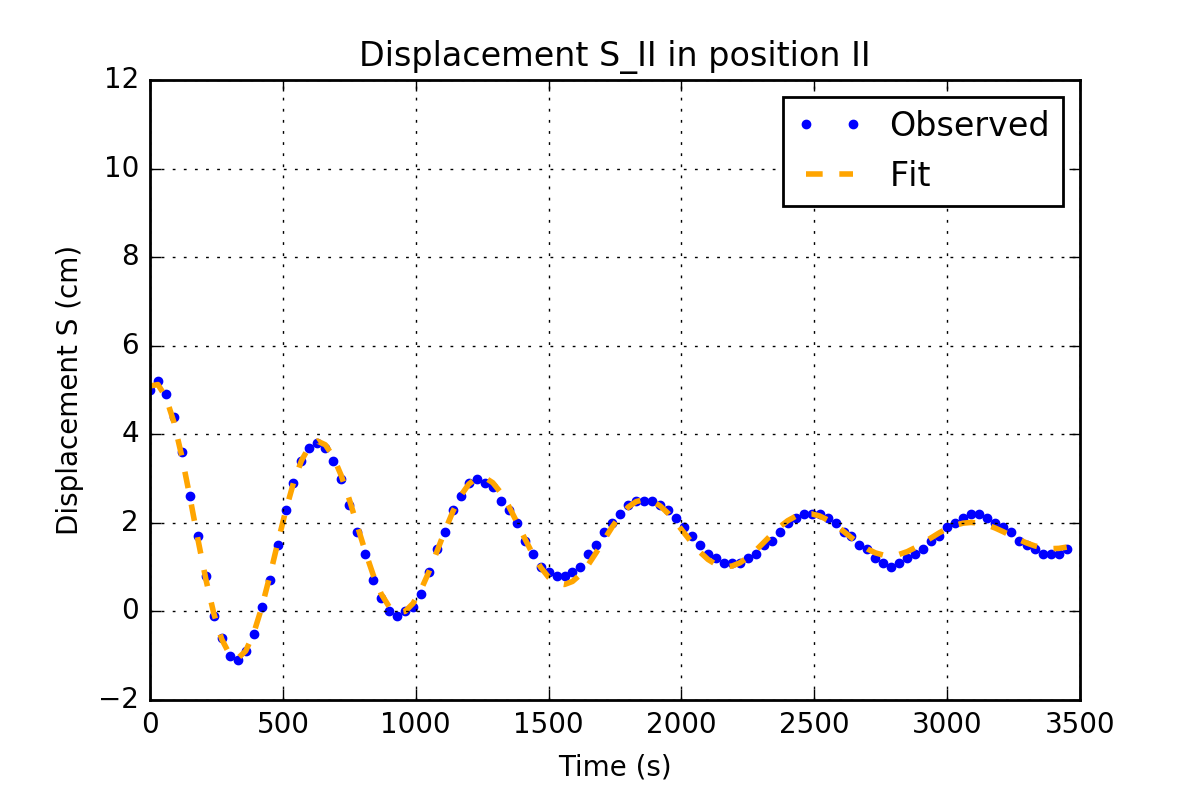
\includegraphics{pos2_datafit}}
  \end{center}
  \caption{Data points and fit function for Position II data}
\end{figure}
\label{fig:pos2_plot}

Similar to the aquired data from Position I, the same procedure is applied to data in Position 2.

\begin{table}[H]
\caption{Optimized fit function parameters for Position II}
\centering
\begin{tabular}{llr}
\toprule
\cmidrule(r){1-2}
Parameter & Value \\
\midrule
$ A$ & $ 5.53 \pm 0.04 $ \\
$ \tau$ & $ 1307 \pm 24 $ \\
$ T$ & $ 614.6 \pm 0.9 $ \\
$ \phi$ & $ -0.26 \pm 0.013 $ \\
$ C$ & $ 1.68 \pm 0.9 $ \\
\bottomrule
\end{tabular}
\end{table}

Thus, from the optimized parameters we find that $S_{I} = 9.74 \pm 0.04$ cm
and $S_{II} = 1.68 \pm 0.01$ cm. Since two different periods were obtained
from the fits we take the average of both and conclude the period of the torsion
balance to be $T= 598 \pm 4$ seconds.

%------------------------------------------------
\section{Analysis}

After all data was collected and and measurements carried out we now compute our estimate for the gravitational
constant G. Below is a summary of all measurements with their corresponding uncertainties.

\begin{table}[H]
\centering
\begin{tabular}{llr}
\toprule
\cmidrule(r){1-2}
Parameter & Value \\
\midrule
$\ L_{0}$ & $ 5.53 \pm 0.04 $ m \\
$\ L_{1}$ & $ 1307 \pm 24 $ cm \\
$\ S_{I}$ & $ 614.6 \pm 0.9 $ cm \\
$\ S_{II}$ & $ -0.26 \pm 0.013 $ cm \\
$\ T$ & $ 1.68 \pm 0.9 $ s \\
\bottomrule
\end{tabular}
\caption{Summary of measurements}
\end{table}

Using these measurements and the given values in the experiment we estimate G by using Equation
\ref{eq:final_g}. Thus, our exprimental estimate for G is,

\begin{equation}
\label{eq:g_measured}
  G_{measured} = 7.68 \cdot 10^{-11} m^3kg^-1s^2
\end{equation}

Via error propagation, the uncertainty of G is given by,

\begin{equation}
\label{eq:final_g}
  \delta G_{measured} = 0.22 \cdot 10^{-11} m^3kg^-1s^2
\end{equation}

Thus, our final reportable estimate for G is,

\begin{equation}
\label{eq:g_measured}
  \boxed{G = (7.7 \pm 0.2)\cdot 10^{-11} m^3kg^{-1}s^2}
\end{equation}

The actual value of G to the same number of significant digits as our estimate is,

\begin{equation}
\label{eq:actual_g}
  G_{actual} = 6.7 \cdot 10^{-11} m^3kg^-1s^2
\end{equation}

Thus, using the actual value of G we quantify the $\%$ error from our estimate as,

$$
 \% \quad error = \frac{\abs{G_{measured} - G_{actual}}}{G_{actual}} \cdot 100 \approx 15\%
$$

%------------------------------------------------

\section{Discussion}

An estimate of G has been obtained with $15\%$ error. While the error is not relatively enormous a much better
estimate could be achieved by more careful experimentation. There are several sources of error that could explain
the obtain error percentage.

One type of error in th experiment was the additional modes of oscillation in the torsion balance. In this experiment
the mode of interest was only the rotational. However, shifting the position of the two large masses would initially
cause other modes that could effect the results.

Another source of error in the experiment is the configuration of the measuring devices. Particularly, the placement of the
glass ruler was difficult to configure and systematic errors could have croped up in the process.


%----------------------------------------------------------------------------------------
%	REFERENCE LIST
%----------------------------------------------------------------------------------------

\begin{thebibliography}{99} % Bibliography - this is intentionally simple in this template

\bibitem[1]{Caldwell:1}
Caldwell, Louis H. (1996)
\newblock Magnetic Damping: Analysis of an Eddy Current Brake Using an Airtrack.
\newblock {\em American Journal of Physics}, Vol 64, No 7.


\bibitem[2]{Leybold:2}
Leybold Didactic GmbH
\newblock Torsion Pendulum (346 00)
\newblock {\em Instruction Sheet 346 00}, 05/99-V5-Sel

\bibitem[3]{Wiki:3}
Wikipedia.
\newblock Cavendish Experiment.
\newblock Wikimedia Foundation, 17 Apr. 2017. Web. 02 May 2017.

\end{thebibliography}

%----------------------------------------------------------------------------------------

\end{document}
